\begin{figure*}[t]
\centering
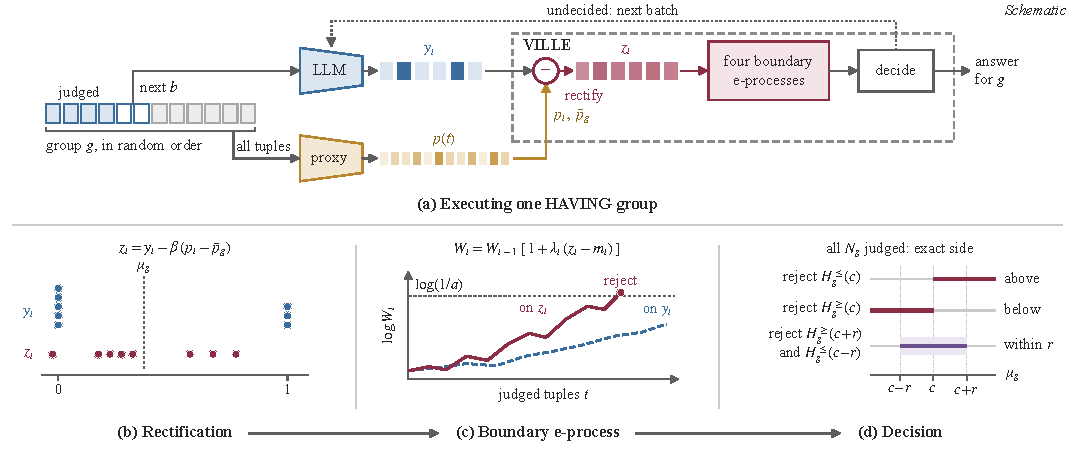
\includegraphics[width=\textwidth]{figures/overview_mechanism.pdf}
\caption{\sys{} executing one HAVING group. (a) In one random order, the LLM judges the next $b$ tuples, the proxy scores all tuples once, and \sys{} rectifies the judgments and updates four boundary e-processes until a decision is certified. (b) Rectification keeps the group mean $\mu_g$ for any proxy, and an informative proxy pulls 0/1 judgments toward it (eight tuples, $\beta=1$). (c) Each e-process bets against the remaining-population null mean $m_t$ (\Cref{eq:mt}) and rejects at wealth $1/a$, $a=\alpha/(2K)$; betting on $y_t$ (dashed) is slower. (d) Rejections that certify each answer; an exhausted group is decided exactly.}
\label{fig:overview}
\end{figure*}
